\documentclass{article}
\usepackage{graphicx} % Required for inserting images
\usepackage{graphicx}
\usepackage{float}
\usepackage{amsmath}
\usepackage{booktabs}
\usepackage{enumitem}
\usepackage{hyperref}
\usepackage{pifont} 

% ----------------------- Packages -----------------------
\usepackage[margin=1in]{geometry}
\usepackage{graphicx}
\usepackage{float}
\usepackage{amsmath}
\usepackage{amssymb}
\usepackage{booktabs}
\usepackage{multirow}
\usepackage{array}
\usepackage{enumitem}
\usepackage{xcolor}
\usepackage{hyperref}
\hypersetup{
  colorlinks = true,
  linkcolor  = blue!55!black,
  citecolor  = blue!55!black,
  urlcolor   = blue!55!black
}
\usepackage{tikz}
\usetikzlibrary{shapes.geometric, arrows.meta, positioning, fit, calc, backgrounds}

% ----------
\hypersetup{colorlinks=true, linkcolor=blue!55!black, citecolor=blue!55!black, urlcolor=blue!55!black}
\title{Fault Before Failure: Multi-Method Anomaly Detection in a Smart Street Lighting Network}

% -------- NEW --------
\documentclass{article}

% ----------------------- Packages -----------------------
\usepackage[margin=1in]{geometry}
\usepackage{graphicx}
\usepackage{float}
\usepackage{amsmath}
\usepackage{amssymb}
\usepackage{booktabs}
\usepackage{multirow}
\usepackage{array}
\usepackage{enumitem}
\usepackage{xcolor}
\usepackage{pifont}
\usepackage{hyperref}
\hypersetup{
  colorlinks = true,
  linkcolor  = blue!55!black,
  citecolor  = blue!55!black,
  urlcolor   = blue!55!black
}
\usepackage{tikz}
\usetikzlibrary{shapes.geometric, arrows.meta, positioning, fit, calc, backgrounds}

\title{Fault Before Failure: A Multi-Paradigm Anomaly Detection Framework for a Smart Street Lighting Feeder}

\author{}
\date{April 2026}

\begin{document}


\maketitle

\begin{abstract}
Urban street lighting networks operate under highly regular temporal schedules, a property that makes their smart-metering records well suited to data-driven anomaly detection but that also makes single-method approaches inherently limited. This study analyzes $14$ months of hourly electricity consumption records ($10{,}214$ retained hourly observations over $424$ days, corresponding to one feeder line in the Avc{\i}lar district of Istanbul) obtained from the Automated Meter Reading system (OSOS) of the regional electricity distribution operator. Rather than committing to a single detection paradigm, we apply four complementary methods: (A)~unsupervised Isolation Forest on hourly observations, (B)~Gramian Angular Field (GAF) image representations combined with an autoencoder for daily structural deviation scoring, (C)~a three-tier ensemble pipeline that fuses STL residual scoring, Isolation Forest at the daily level, and PELT change-point detection, and (D)~a supervised Gradient Boosting model that predicts failures within a $24$-hour horizon from a merged energy--electrical feature set. All four methods operate on a shared preprocessed dataset to enable fair comparison. We show that each approach surfaces a different slice of the same operational reality: hourly Isolation Forest captures switching-transition irregularities; GAF detects sustained multi-week structural drift; the three-tier ensemble provides calibrated daily severity and localizes regime shifts; and the supervised model ranks pre-failure hours by risk. The observed quantitative scores, which are modest in absolute terms, are interpreted with respect to fundamental data-observability limits: five of six labeled outages occurred during daylight hours when lamps are off and therefore leave no signature in consumption, and the positive class represents only $5.59\%$ of observations. The results indicate that the practical value of such a system lies in the \emph{union} of complementary flags rather than in the headline score of any single model.

\end{abstract}

\section{Introduction}
Urban street lighting systems constitute a critical component of municipal infrastructure, operating continuously under highly structured temporal schedules. Under normal conditions, their electricity consumption follows a predictable daily pattern: a stable load during nighttime hours when luminaires are active, near-zero consumption during daylight, and sharp transitions at the evening switch-on and morning switch-off periods. This regularity makes street lighting networks particularly well suited to data-driven anomaly detection~\cite{nespoli2024street,ptacek2022road}: deviations from the expected consumption profile are inherently meaningful and can serve as early indicators of equipment malfunction, relay failure, or communication irregularities in the remote management system.

For large-scale operators, such as the electricity distribution company under study, which manages one of the largest urban lighting networks on the European side of Istanbul, maintaining operational reliability across thousands of distributed field units is a significant challenge. Manual inspection of consumption records is neither scalable nor timely; by the time a fault is identified through routine maintenance, service interruptions may already have occurred. Automated anomaly detection offers a more systematic alternative~\cite{himeur2021survey,wang2020review}: by continuously monitoring consumption data against learned baselines, deviations can be flagged as they occur, enabling targeted intervention before failures escalate.

\subsection*{Research Question and Scope}
This study analyzes $14$ months of hourly electricity consumption data obtained from the Automated Meter Reading System (OSOS) of the electricity distribution operator serving the European side of Istanbul, covering the period from January~$2025$ to February~$2026$. The primary research question is:
 
\begin{quote}
\emph{Given real-world smart-metering data with limited ground truth, unknown fault semantics, and strong seasonal non-stationarity, can a combination of complementary anomaly detection paradigms --- statistical, unsupervised machine learning, structural image-based, and supervised --- produce a more operationally useful picture of the lighting network than any single method on its own?}
\end{quote}

\subsection*{Justification of the Multi-Paradigm Framework}
A recurring observation in the anomaly-detection literature~\cite{chandola2009anomaly,aggarwal2017outlier,aggarwal2017ensemble} is that no single detector captures every fault type. Point-level detectors miss slowly accumulating drift; change-point detectors miss isolated spikes; supervised models miss novel failure modes; purely unsupervised methods cannot exploit even the limited ground truth that is available. Rather than choosing one detector and absorbing its blind spots, this study intentionally places four methods side by side on the same cleaned dataset and compares what each one surfaces. The four methods were selected to span three orthogonal axes:

\begin{enumerate}[leftmargin=1.5em,itemsep=1pt]
  \item \textbf{Temporal resolution:} hourly (Isolation Forest) vs.\ daily (GAF, three-tier ensemble, supervised).
  \item \textbf{Supervision:} fully unsupervised (Isolation Forest, GAF), ensemble of unsupervised signals (three-tier pipeline), and supervised (Gradient Boosting).
  \item \textbf{Representation:} raw numerical features (Isolation Forest, supervised), image-based structural encoding (GAF), and decomposition-based residual analysis (STL, change-points).
\end{enumerate}
In the data set analyzed, no single method recovers all four key operational events: the March 2025 sudden-drop cluster, the February 2026 complete blackout, the December 2025 progressive degradation, and the 12 May 2025 nighttime outage are each surfaced by a different subset of the four detectors.

\subsection*{Contributions}
This work offers three contributions:

\begin{itemize}[leftmargin=1.5em,itemsep=1pt]
  \item A unified preprocessing and evaluation protocol under which four distinct anomaly detection approaches are applied to the same real-world smart-metering dataset, enabling comparison rather than isolated reporting.
  \item A demonstration that the four methods are \emph{complementary} rather than competitive: the union of flags captures events that no single detector identifies alone, while agreement among detectors provides an empirical confidence signal.
  \item A quantitative and literature-grounded interpretation of why supervised detection on this task produces modest absolute scores, situating the observed numbers within known limitations of imbalanced classification~\cite{saito2015precision,hand2009measuring} and data observability on short, single-line field datasets.
\end{itemize}

% =====================================================================
\section{Related Work}\label{sec:related}
% =====================================================================
Anomaly detection has been studied extensively across statistics, machine learning, and signal processing~\cite{chandola2009anomaly,hodge2004survey,aggarwal2017outlier,hawkins1980identification}. In the energy and smart-metering context, the literature broadly falls into four families that correspond closely to the four approaches adopted in this study.

\paragraph{Statistical residual and control-chart methods.}
Classical approaches decompose a time series into trend, seasonal, and residual components and flag the residual using robust statistical tests. STL decomposition~\cite{cleveland1990stl} is widely used because it tolerates outliers in a robust variant and accommodates non-integer seasonalities. Residual-level outlier detection with the Modified Z-Score~\cite{iglewicz1993outliers} is preferred over the classical z-score in the presence of a heavy-tailed residual because the MAD statistic is not inflated by the very outliers one wishes to detect. For gradually emerging deviations, cumulative sum control charts~\cite{page1954cusum} accumulate evidence over time and react to small but persistent departures from expected behavior.

\paragraph{Unsupervised machine learning.}
Isolation Forest~\cite{liu2008isolation,liu2012isolation} has become a standard tabular anomaly detector because it achieves linear computational cost via sub-sampling, imposes no distributional assumptions, and is robust to high-dimensional feature spaces. Density-based alternatives such as LOF~\cite{breunig2000lof} remain competitive in low dimensions but scale less favorably. Neural reconstruction models such as LSTM-based autoencoders~\cite{malhotra2016lstm} learn sequence-level normality and flag sequences that the decoder fails to reproduce.

\paragraph{Image-based representations of time series.}
Time-series-to-image transformations such as the Gramian Angular Field~\cite{wang2015gaf,wang2015imaging} encode a one-dimensional temporal vector as a two-dimensional matrix whose entries summarize pairwise angular relationships among values. This permits the use of image-domain tools --- notably convolutional or autoencoder models --- to score \emph{structural} rather than \emph{point-level} deviations. The method has been applied to classification of industrial signals and has subsequently been adopted for anomaly analysis where a single day or cycle is the semantic unit of interest.

\paragraph{Change-point detection.}
Where the above methods score \emph{per-observation} anomalies, change-point methods such as PELT~\cite{killick2012pelt} and related offline procedures surveyed by~\cite{truong2020ruptures,aminikhanghahi2017survey} localize the specific time indices at which the \emph{generative parameters} of the series change. In a maintenance context, this corresponds to partial bulb loss, circuit reconfiguration, or bulk replacement --- all of which manifest as a level shift rather than an isolated spike.

\paragraph{Supervised failure prediction on tabular data.}
When partial labels are available, supervised classification shifts the problem from ``what is unusual'' to ``what precedes a known failure.'' Gradient Boosting Decision Trees~\cite{friedman2001gbm,chen2016xgboost} remain state of the art on small to mid-sized tabular datasets~\cite{shwartz2022tabular}. On heavily imbalanced label distributions, synthetic oversampling methods such as SMOTE~\cite{chawla2002smote}, SMOTE+Tomek~\cite{batista2004study}, and ADASYN~\cite{he2008adasyn} are the standard recipe; however, the oversampling literature itself~\cite{fernandez2018smote} is explicit that threshold tuning on the original distribution is often competitive. Reliable evaluation on imbalanced problems requires careful choice of metrics: precision--recall curves~\cite{saito2015precision} and metric-aware assessments~\cite{hand2009measuring,fawcett2006roc} are preferred over a naive accuracy or even ROC-AUC.

\paragraph{Position of this work.}
Each family above has been applied to street-lighting or building-energy anomaly detection in isolation~\cite{nespoli2024street,ptacek2022road,himeur2021survey,wang2020review}. The distinctive contribution of this study is not the introduction of any new detector but the \emph{parallel application and comparison} of four mature paradigms on the same real-world dataset, under a shared preprocessing protocol and a consistent evaluation framework.

% =====================================================================
\section{Dataset}\label{sec:dataset}
% =====================================================================

\subsection{Source and Scope}
The primary dataset consists of hourly active power withdrawal measurements recorded by the OSOS (\emph{Otomatik Say{a}{\c c} Okuma Sistemi}, ``Automated Meter Reading System'') maintained by the regional electricity distribution operator serving the European side of Istanbul. The data correspond to a single urban street-lighting feeder line (identifier~\texttt{2193681000}) in the Avc{\i}lar district. Data were supplied as one Excel workbook per calendar month; the observation window spans January~$2025$ to February~$2026$, yielding $14$ monthly files.

In the raw files each row encodes one month, and the day-of-month values are spread across columns, with each hourly bin (\texttt{00-01}, \texttt{01-02}, \ldots, \texttt{23-24}) represented as a separate column. Both \emph{withdrawal} (energy consumed by the network) and \emph{feed-in} (bidirectional metering artifacts) readings appear in the source; only \emph{withdrawal} records were retained, because only these reflect the energy actually drawn by the lighting network.

\subsection{Scale}
After restructuring (Section~\ref{sec:preprocessing}) and removal of invalid calendar entries and row duplicates, the shared cleaned dataset used by all four approaches contains:

\begin{itemize}[leftmargin=1.5em,itemsep=0pt]
  \item $10{,}214$ retained hourly observations at $1$-hour resolution;
  \item $424$ daily aggregates over the $14$-month window (Jan $2025$ -- Feb $2026$);
  \item $19$ engineered features at the daily level and up to $53$ features at the hourly level (see Section~\ref{sec:preprocessing}).
\end{itemize}

\subsection{Secondary Datasets}
In addition to the primary hourly consumption record, three secondary datasets provided by the operator were used in specific sub-analyses:

\begin{itemize}[leftmargin=1.5em,itemsep=1pt]
  \item \texttt{rpt-300 --- Sayaç Kesinti Raporu} (``Meter Outage Report'') lists $7$ meter-side outage events on $6$ unique calendar days, with start and end timestamps.
  \item \texttt{rpt-301 --- Modem Kesinti Raporu} (``Modem Outage Report'') lists $28$ communication interruption events, used  as the target variable to train the supervised learning model.
  \item \texttt{Ak{\i}m--Gerilim Raporu} (``Current--Voltage Report'') provides three-phase current and voltage measurements over the same period, used by the supervised approach to construct electrical-domain features ($9{,}456$ hourly records merged with $9{,}780$ hourly energy records on shared timestamps).
\end{itemize}

\subsection{Ground Truth}
\label{subsec:groundtruth}

Due to the different methodological requirements of the analytical pipelines, two distinct sets of ground truth labels were utilized in this study. For evaluating the unsupervised anomaly detection models (e.g., the Three-Tier Ensemble), the \texttt{rpt-300} report was used, providing the operator-verified physical meter fault labels. Its entries were aggregated to the day level, yielding $6$ labeled outage days. An essential characteristic of this label set is that \textbf{five of the six outages occurred during daylight hours, when the lamps are off and no electricity is drawn by the network in normal operation}. Consequently, most labeled physical outages leave essentially no signature in the consumption series---a data-observability limit that inherently bounds the recall of unsupervised methods. Conversely, because $6$ positive instances are fundamentally insufficient to train a supervised machine learning model, the supervised Gradient Boosting approach utilized the $28$ communication interruption events from the \texttt{rpt-301} report as its target variable. This yielded $547$ pre-failure hourly observations, providing the supervised model with the necessary sample size to learn discriminative patterns for predicting impending communication and modem losses rather than physical meter failures.


\subsection{Known Data Quality Issues}
\label{subsec:quality}
Two systematic data-quality issues were identified in the raw files and resolved during preprocessing:

\begin{enumerate}[leftmargin=1.5em,itemsep=2pt]
  \item \textbf{Duplicate daily totals.} The raw \texttt{23-24} hourly bin for certain days contained values near $99$~kWh, corresponding to the daily total rather than an hourly reading; these were de-duplicated by collapsing on the reconstructed timestamp.
  \item \textbf{Invalid calendar dates.} The raw Excel exports contained day-$29$--$31$ rows for months without these days (e.g., February~$29$ in a non-leap year, April/June/September/November day $31$); these $10$ rows were removed after validation against \texttt{calendar.monthrange}.
\end{enumerate}

Additional gaps arose from communication losses between the meter and the OSOS backend: the expected $424 \times 24 = 10{,}176$ hourly rows contained approximately $380$ missing entries prior to imputation. Their treatment is described in Section~\ref{subsec:missing}.
% =====================================================================
\section{Data Preprocessing}\label{sec:preprocessing}
% =====================================================================
All four approaches operate on a single shared preprocessed dataset, ensuring that performance differences cannot be attributed to discrepancies in data cleaning. The raw data, initially provided in a wide format with days as columns, was restructured into a long format where each row corresponds to a single hourly observation indexed by a fully resolved \texttt{pandas.Timestamp}, reconstructed from the period (\texttt{MM/YYYY}), day-of-month, and hour-bin columns by taking the lower bound of each bin (e.g.\ \texttt{``17--18''} $\rightarrow$ hour $17$). During this restructuring, only records tagged as energy withdrawal were retained, as feed-in measurements reflect bidirectional metering artifacts rather than the physical energy drawn by the lighting network. Duplicate timestamps originating from daily-total artifacts (Section~\ref{subsec:quality}) and rows corresponding to non-existent calendar dates were removed via \texttt{drop\_duplicates} and validation against \texttt{calendar.monthrange}, respectively.

Missing hourly observations were addressed using a duration-aware strategy consistent with established practices~\cite{littlerubin2019}. Short gaps ($\leq 3$ consecutive hours) were resolved via time-based linear interpolation, as these typically represent transient communication-layer artifacts; interpolating preserves temporal continuity without fabricating artificial zero-consumption anomalies. In contrast, long gaps ($>3$ consecutive hours) were explicitly flagged (\texttt{has\_imputed\_long=1}) and assigned a value of zero, reflecting the operational reality that sustained data loss is often indicative of a true meter or network failure --- imputing a reconstructed value in this regime would fabricate operational history. For its structural analysis, the GAF pipeline additionally applied monthly hourly median imputation, replacing a missing value at hour $h$ in month $m$ with the median value of hour $h$ over month $m$, which respects seasonally shifting sunset/sunrise timing without distorting it.

Depending on the temporal resolution of the specific analytical approach, data was subsequently engineered at either the daily or hourly level. For the daily-level models (GAF, the three-tier ensemble, and parts of the supervised pipeline), observations were aggregated per calendar day, with operationally active hours identified using a $\geq 1.0$~kWh threshold. This cutoff is empirically grounded in the strongly bimodal hourly withdrawal distribution: a large daytime mode below $0.05$~kWh (lamps off, only standby draw), an active nighttime mode at $6$--$7$~kWh, and a near-empty band between $0.1$ and $1$~kWh populated almost exclusively by switching-transition hours. Placing the cutoff at $1.0$~kWh therefore separates inactive from active hours along the natural valley of the distribution and tracks seasonal sunrise/sunset shifts automatically, without requiring a hard-coded astronomical schedule. The resulting $19$-column feature space (Table~\ref{tab:daily_features}) is built around rolling \emph{medians}---robust to the very outliers one is trying to detect---over a $28$-day baseline window, chosen as long enough to track seasonal drift but short enough not to over-smooth (a $7$-day window underfits seasonality, while a $90$-day window fails to capture the autumn-to-winter onset), and is complemented by sinusoidal cyclic encodings of month and day-of-year, which preserve the operational contiguity of December and January that a naive integer encoding would destroy. Conversely, the hourly Isolation Forest and supervised Gradient Boosting models utilize an hourly feature space combining cyclical encodings of time, $24$-hour lag components, and rolling statistics over $3$-, $6$-, $12$-, and $24$-hour windows. When merged with the electrical-domain measurements, the supervised feature set expands to $53$ variables, incorporating phase-current imbalance ($\sigma_I = \mathrm{std}(I_R, I_S, I_T)$), voltage imbalance, average power factor, apparent and active power, and the energy-to-current ratio. Across all pipelines, robust scaling (median/IQR) was preferred over standard scaling to prevent outlier-heavy periods from distorting the normalized distributions.

The complete preprocessing pipeline, including explicit missing-value handling and deterministic scaler fitting on training splits only, is implemented in \texttt{src/scripts/preprocess.py} and \texttt{ground\_truth.py}, and can be reproduced end-to-end from the raw operator Excel files via \texttt{python src/scripts/run\_pipeline.py --tiers 1,2,3}.

\begin{table}[H]
\centering
\caption{Daily features available to all daily-level approaches (shared preprocessing output)}
\label{tab:daily_features}
\small
\begin{tabular}{p{3.3cm}p{5.5cm}p{5.2cm}}
\toprule
\textbf{Feature} & \textbf{Definition} & \textbf{Purpose}\\
\midrule
\texttt{daily\_active\_kwh}      & Sum of withdrawal over hours with $\geq 1$~kWh & Primary anomaly signal\\
\texttt{active\_hours\_count}    & Number of hours above the active threshold & Partial-fault signal\\
\texttt{mean\_active\_intensity} & Mean kWh per active hour & Current-drop indicator\\
\texttt{p10\_active}             & $10$th percentile over active hours & Detects brief collapses\\
\texttt{night\_missing\_frac}    & Fraction of hours with $<0.5$~kWh & Missing-night indicator\\
\texttt{rolling\_28d\_median}    & $28$-day rolling median of \texttt{daily\_active\_kwh} & Seasonal baseline\\
\texttt{daily\_kwh\_norm}        & Ratio to rolling baseline & Season-normalized value\\
\texttt{delta\_1d}, \texttt{delta\_7d} & $1$- and $7$-day differencing & Abrupt-change capture\\
\texttt{rolling\_7d\_std}        & $7$-day rolling standard deviation & Volatility\\
\texttt{rolling\_28d\_zscore}    & z-score against $28$-day window & Normalized anomaly score\\
\texttt{month\_sin/cos}          & Sinusoidal encoding of month & Seasonal context for ML\\
\texttt{day\_of\_year\_sin/cos}  & Sinusoidal encoding of day-of-year & Within-year position\\
\bottomrule
\end{tabular}
\end{table}


\section{Methodology}
This section presents the four anomaly-detection approaches that operate on the shared cleaned dataset described in Section~\ref{sec:dataset} and the shared preprocessing pipeline of Section~\ref{sec:preprocessing}. The four approaches were selected to cover orthogonal regions of the design space (resolution, supervision, representation; cf.\ Section~1), and they are introduced below in the order in which they appear in the pipeline diagram of Figure~\ref{fig:flowchart}: hourly Isolation Forest (Approach~A), Gramian Angular Field with autoencoder (Approach~B), the three-tier ensemble (Approach~C), and supervised Gradient Boosting (Approach~D).

% ───────────────────────────────────────────── FEZA methodology
The Gramian Angular Field (GAF) approach was adopted as a pattern-based anomaly detection method that treats each day’s electricity consumption as a complete 24-hour structure rather than as isolated hourly measurements. By converting daily consumption vectors into two-dimensional image representations, the method captures temporal relationships across the full day and enables the detection of structural deviations from expected street-lighting operation. This makes the GAF-based analysis particularly suitable for identifying abnormal daily patterns that may not be apparent from point-level observations alone. The full technical pipeline, including preprocessing, image transformation, anomaly scoring, and data-quality handling, is provided in Section 2.3.

% ───────────────────────────────────────────── FEZA methodology en

\subsection{Design Philosophy: Four Complementary Perspectives}
\label{subsec:design}

Building on the multi-paradigm motivation introduced in Section~1, this subsection translates that motivation into a concrete operational framing: each of the four detectors makes an implicit assumption about the \emph{form} that an anomaly takes, and Table~\ref{tab:four_perspectives} maps each approach onto the class of operational event for which its assumption is naturally valid. A point outlier at a given hour is the target of Approach~A (hourly Isolation Forest); a distorted daily structure is the target of Approach~B (GAF + autoencoder); a daily-level deviation from a statistical baseline with confirmatory change-point is the target of Approach~C (three-tier ensemble); and a pattern that precedes a labelled failure is the target of Approach~D (supervised Gradient Boosting). When all four assumptions are simultaneously valid, the event is surfaced with high confidence across methods; when only one assumption is valid, only the corresponding method flags it, and this specificity is itself useful because it characterises the \emph{type} of event encountered.


Table~\ref{tab:four_perspectives} summarizes how the four approaches partition the design space and which classes of event each one is primarily sensitive to.

\begin{table}[H]
\centering
\caption{The four approaches positioned along three orthogonal axes. Each one is sensitive to a different class of operational anomaly}
\label{tab:four_perspectives}
\small
\begin{tabular}{lcccc}
\toprule
& \textbf{Approach A} & \textbf{Approach B} & \textbf{Approach C} & \textbf{Approach D}\\
& \emph{hourly iForest} & \emph{GAF + AE} & \emph{3-tier ensemble} & \emph{supervised GBDT}\\
\midrule
Resolution     & hourly  & daily   & daily   & hourly\\
Supervision    & unsup.  & unsup.  & unsup.\ ensemble & supervised\\
Representation & tabular & image   & tabular + residual + CP & tabular\\
Primary target & switching irregularities & structural daily drift & daily deviations \& regime shifts & $24$-hour pre-failure\\
\bottomrule
\end{tabular}
\end{table}

The end-to-end relationship of the four approaches to the shared preprocessing stage and to the cross-model benchmark is shown in the pipeline diagram of Figure~\ref{fig:flowchart}.



% -------- Flowchart --------
\begin{figure}[H]
\centering
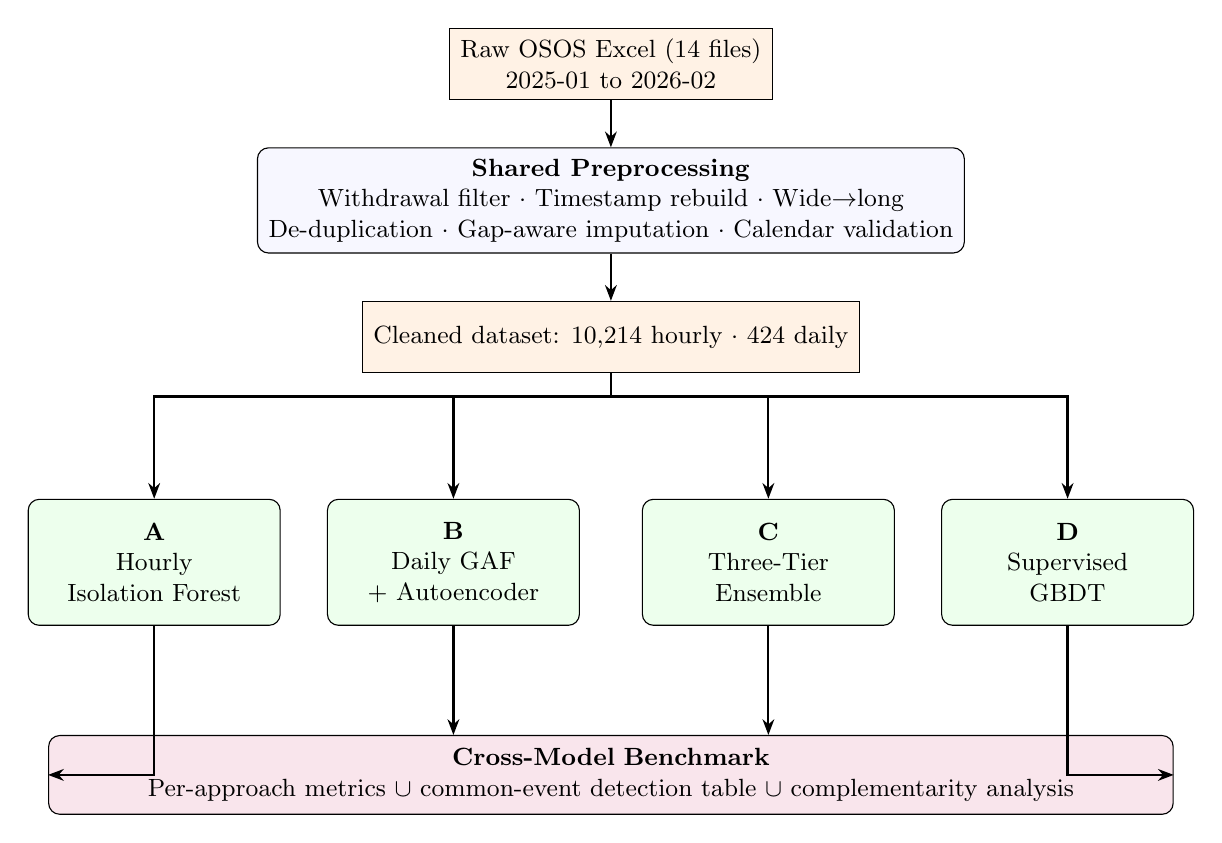
\begin{tikzpicture}[
  node distance=6mm and 10mm,
  font=\small,
  box/.style  ={rectangle, rounded corners, draw, align=center, minimum height=9mm, inner sep=4pt, fill=blue!3},
  data/.style ={rectangle, draw, align=center, minimum height=9mm, inner sep=4pt, fill=orange!10},
  model/.style={rectangle, rounded corners, draw, align=center, minimum height=16mm, inner sep=4pt, fill=green!7, minimum width=32mm},
  final/.style={rectangle, rounded corners, draw, align=center, minimum height=10mm, inner sep=4pt, fill=purple!10, text width=140mm},
  arr/.style  ={-{Stealth[length=2mm]}, thick}
  ]

  \node[data]  (raw)    {Raw OSOS Excel (14 files)\\$2025\text{-}01$ to $2026\text{-}02$};
  \node[box, below=of raw] (pre) {%
    \textbf{Shared Preprocessing}\\
    Withdrawal filter~$\cdot$~Timestamp rebuild~$\cdot$~Wide$\to$long\\
    De-duplication~$\cdot$~Gap-aware imputation~$\cdot$~Calendar validation};
  \node[data, below=of pre] (clean) {Cleaned dataset: $10{,}214$ hourly~$\cdot$~$424$ daily};

  \node[model, below=16mm of clean, xshift=-58mm] (ma) {\textbf{A}\\Hourly\\Isolation Forest};
  \node[model, below=16mm of clean, xshift=-20mm] (mb) {\textbf{B}\\Daily GAF\\+ Autoencoder};
  \node[model, below=16mm of clean, xshift=20mm]  (mc) {\textbf{C}\\Three-Tier\\Ensemble};
  \node[model, below=16mm of clean, xshift=58mm]  (md) {\textbf{D}\\Supervised\\GBDT};

  \node[final, below=46mm of clean] (res) {%
    \textbf{Cross-Model Benchmark}\\
    Per-approach metrics $\cup$ common-event detection table $\cup$ complementarity analysis};

  \draw[arr] (raw)  -- (pre);
  \draw[arr] (pre)  -- (clean);
  \draw[arr] (clean.south) -- ++(0,-3mm) -| (ma.north);
  \draw[arr] (clean.south) -- ++(0,-3mm) -| (mb.north);
  \draw[arr] (clean.south) -- ++(0,-3mm) -| (mc.north);
  \draw[arr] (clean.south) -- ++(0,-3mm) -| (md.north);
  \draw[arr] (ma.south) |- (res.west);
  \draw[arr] (mb.south) -- (res.north -| mb.south);
  \draw[arr] (mc.south) -- (res.north -| mc.south);
  \draw[arr] (md.south) |- (res.east);

\end{tikzpicture}
\caption{End-to-end pipeline of the study. A single shared preprocessing stage feeds four parallel analytical streams (A--D); their outputs are recombined in the cross-model benchmark. The diagram is the visual counterpart of the ``four complementary perspectives'' argument developed in Section~\ref{subsec:design}}
\label{fig:flowchart}
\end{figure}

% =====================================================================
% ---------------------------- SENA'S MODEL------------------------

\subsection{Isolation Forest-Based Anomaly Detection}
\label{subsec:iforest_hourly}
\subsubsection{Algorithm Selection}

Isolation Forest was selected as the anomaly detection algorithm for
this study for three principal reasons. First, the absence of verified
fault records in the OSOS dataset made supervised approaches
inapplicable; Isolation Forest operates in a fully unsupervised
manner, requiring no labeled examples of anomalous
behavior~\cite{liu2008isolation}. Second, the algorithm achieves
linear time complexity through sub-sampling and constructs its
ensemble of random decision trees without relying on distance or
density computations, making it computationally efficient on large
time-series datasets~\cite{liu2012isolation}. Third, it imposes no
assumption on the underlying data distribution, making it well-suited
to the irregular consumption patterns characteristic of street
lighting systems~\cite{chandola2009anomaly, ptacek2022road,
nespoli2024street}.

The algorithm operates on the principle that anomalous observations
are \textit{``few and different''}: in a forest of randomly
constructed decision trees, anomalous data points reach leaf nodes in
significantly fewer partitions than typical observations, yielding
shorter average path lengths and correspondingly lower anomaly
scores~\cite{liu2008isolation}. The key hyperparameters used in this
study are summarized in Table~\ref{tab:if_params}.

\begin{table}[h]
\centering
\caption{Isolation Forest Hyperparameter Configuration}
\label{tab:if_params}
\begin{tabular}{lll}
\hline
\textbf{Parameter} & \textbf{Value} & \textbf{Justification} \\
\hline
\texttt{n\_estimators}  & 200  & Ensemble stability across large dataset \\
\texttt{contamination}  & 0.03 & Selected via sensitivity sweep (Table~\ref{tab:contamination_sweep}); \\
                        &      & consistent with observed seasonal anomaly rates \\
\texttt{random\_state}  & 42   & Reproducibility \\
\hline
\end{tabular}
\end{table}

The \texttt{contamination} parameter was selected via a systematic
sensitivity sweep over the candidate set $\{0.01, 0.03, 0.05, 0.10\}$,
with results summarized in Table~\ref{tab:contamination_sweep}. A value
of 0.03 was retained because it produces a flagged rate consistent with
the seasonal breakdown in Table~\ref{tab:seasonal}: non-winter months
exhibit low anomaly rates (0.6\%--1.6\%), while the winter period reaches
5.4\%, yielding a dataset-wide average near 3\%. Higher contamination
values (0.05--0.10) over-flag stable autumn and spring months; lower
values (0.01) suppress real deviations in the winter window.
 
\begin{table}[h]
\centering
\caption{Contamination Sensitivity Sweep --- Hourly Isolation Forest}
\label{tab:contamination_sweep}
\begin{tabular}{ccc}
\hline
\textbf{Contamination} & \textbf{Anomaly Count} & \textbf{Anomaly Rate (\%)} \\
\hline
0.01 &   99 & 0.97 \\
\textbf{0.03} & \textbf{306} & \textbf{3.01} \\
0.05 &  509 & 5.00 \\
0.10 & 1018 & 10.00 \\
\hline
\end{tabular}
\end{table}

% ─────────────────────────────────────────────
\subsubsection{Feature Engineering}
% ─────────────────────────────────────────────

Raw consumption values alone are insufficient for meaningful anomaly
detection in this context: a value of 7~kWh, for example, is entirely
normal at 02:00 when lights are expected to be on, yet represents a
significant deviation at 14:00 when the network should be drawing
near-zero power. To enable the model to understand this temporal
context, several additional features were derived from the timestamp
index, as described in Table~\ref{tab:features}.

\begin{table}[h]
\centering
\caption{Engineered Features Used in Model Training}
\label{tab:features}
\begin{tabular}{p{3.2cm}p{4.5cm}p{5.5cm}}
\hline
\textbf{Feature} & \textbf{Description} & \textbf{Rationale} \\
\hline
Consumption        & Hourly active power draw (kWh) & Primary anomaly signal \\
\texttt{hour\_sin} & $\sin\!\left(\dfrac{2\pi \cdot h}{24}\right)$ &
  Circular encoding: preserves temporal \\
\texttt{hour\_cos} & $\cos\!\left(\dfrac{2\pi \cdot h}{24}\right)$ &
  continuity between hours 23:00 and 00:00 \\
Day of week        & Integer 0--6 (Mon--Sun) & Captures weekly schedule variation \\
\texttt{lag24}     & Consumption 24 hours prior & Same-hour previous-day baseline; \\
                   &                            & flags abrupt deviations from \\
                   &                            & expected repetitive behavior \\
\hline
\end{tabular}
\end{table}

Sinusoidal encoding was applied to the hour variable because a linear
representation treats hours~23 and~0 as maximally distant, whereas
operationally they are contiguous. The \texttt{lag24} feature exploits
the highly repetitive daily schedule of street lighting systems: since
normal consumption at any given hour closely mirrors the same hour on
the preceding day, a significant departure from \texttt{lag24}
constitutes a direct anomaly signal. All features were standardized
using \texttt{StandardScaler} prior to model fitting.

% ─────────────────────────────────────────────
\subsubsection{Detection Pipeline}
% ─────────────────────────────────────────────

The analysis was conducted under two complementary settings, each
addressing a distinct objective. The global setting applies Isolation
Forest to the full dataset in order to characterize the overall anomaly
distribution across seasons and hours of day. 

The train--test setting examines whether the decision boundary learned
from historical data remains meaningful when transferred to an unseen
future period. Specifically, it evaluates whether the model's notion of
normality, derived primarily from non-winter months, assigns elevated
anomaly scores to winter operating conditions not previously observed
during training.

Because Isolation Forest is fully unsupervised, this second setting
should not be interpreted as predictive performance evaluation in the
supervised sense, since no ground-truth anomaly labels are available to
compute metrics such as precision, recall, or accuracy. Instead, it
serves as a temporal robustness check, assessing whether the learned
boundary responds coherently when applied to a shifted future data
distribution.

\paragraph{Global Anomaly Detection}\mbox{}\\
In the first setting, Isolation Forest was applied across the full
14-month dataset comprising \textbf{10,176 hourly observations}. The
objective was exploratory: to examine the overall distribution of
anomalies, determine whether they clustered during specific periods,
and establish a system-wide baseline. Each observation was classified
as either normal or anomalous, and results were aggregated by month,
day, hour, and meteorological season. This setting yielded
\textbf{306 detected anomalies}, with the seasonal breakdown shown in
Table~\ref{tab:seasonal}.

\begin{table}[h]
\centering
\caption{Seasonal Distribution of Anomalies --- Global Detection}
\label{tab:seasonal}
\begin{tabular}{lccc}
\hline
\textbf{Season} & \textbf{Anomalies} & \textbf{Normal} & \textbf{Anomaly Rate} \\
\hline
Winter   (Dec, Jan, Feb) & 194 & 3{,}382 & 5.4\% \\
Summer   (Jun, Jul, Aug) &  63 & 2{,}145 & 2.9\% \\
Spring   (Mar, Apr, May) &  36 & 2{,}172 & 1.6\% \\
Autumn   (Sep, Oct, Nov) &  13 & 2{,}171 & 0.6\% \\
\hline
\textbf{Total} & \textbf{306} & \textbf{9{,}870} & \textbf{3.0\%} \\
\hline
\end{tabular}
\end{table}

Winter accounted for 63.4\% of all flagged observations. This finding
aligns with expectations: lower temperatures and extended lighting hours
increase the load on network infrastructure, making faults more likely
during this period.

\paragraph{Temporal Holdout Robustness Check}\mbox{}\\
To assess whether the anomaly boundary learned from historical data
remained stable when applied to future unseen observations, the dataset
was split chronologically. All observations prior to December~2025
formed the training set, while the remainder constituted the holdout
period. The \texttt{StandardScaler} normalization was computed on the
training set only and then applied to the holdout set without refitting,
preventing information leakage. This setup approximates a realistic
deployment scenario in which a model trained on historical behavior is
later used to screen newly arriving data. The anomaly counts reported
for the holdout period do not constitute a performance metric --- since
no verified fault labels exist for this period, precision and recall
cannot be computed. The reported figures instead characterize how the
fixed decision boundary responds to the shifted winter operating
distribution. The split statistics are summarized in
Table~\ref{tab:split}.

\begin{table}[h]
\centering
\caption{Temporal Holdout Split Statistics}
\label{tab:split}
\begin{tabular}{lccc}
\hline
\textbf{Set} & \textbf{Observations} & \textbf{Anomalies Detected} &
\textbf{Anomaly Rate} \\
\hline
Training (Jan~2025 -- Nov~2025) & 7{,}992 & --- & --- \\
Holdout  (Dec~2025 -- Feb~2026) & 1{,}786 & 138 & 7.7\% \\
\hline
\end{tabular}
\end{table}

The holdout period anomaly rate of 7.7\% exceeded the nominal 3\%
contamination level specified during training. This should not be
interpreted as model miscalibration. Rather, it is a direct consequence
of the seasonal pattern identified in the global detection setting: the
model learned normality from predominantly non-winter data, and flagged
the December--February holdout period as one exhibiting heightened
operational deviation.

%-----------------------------SENA'S MODEL END----------------------------




%--------------------------Ali Gokay — Three-Tier Ensemble Pipeline
\subsection{Three-Tier Ensemble Anomaly Detection Pipeline}

The three approaches presented above (hourly Isolation Forest, GAF--autoencoder, and the supervised Gradient Boosting prediction described later) each target a single facet of the anomaly-detection problem: point outliers in hourly load, structural deviations in full-day shape, and labelled pre-failure hours respectively. None of them, taken alone, is designed to separate a \emph{one-day sudden drop} from a \emph{multi-week gradual degradation} or from a \emph{permanent regime shift}. Anomaly-detection surveys \cite{chandola2009anomaly,aggarwal2017outlier} and ensemble-based reviews \cite{aggarwal2017ensemble,zhang2023ensemble} repeatedly stress that these failure modes require methodologically different detectors, and that ensembling complementary views is the principled remedy.

The three-tier ensemble pipeline introduced in this subsection is designed around that observation. It operates on the \emph{daily} aggregation of the same 14-month line (424 days $\times$ 18 engineered features) and combines three deliberately different detectors: statistical residual analysis, a multivariate machine-learning detector, and an offline change-point detector. Each tier targets a distinct temporal scale of anomaly, and their scores are fused into a single per-day severity and confidence level.

\subsubsection{Tier 1 --- Statistical Residual Detectors}

The first tier targets \emph{single-day} and \emph{short-burst} deviations and consists of three complementary statistical signals applied to the daily active-hours energy series.

An STL decomposition \cite{cleveland1990stl} with an annual period and the robust variant is first used to separate long-term trend, yearly seasonality, and residuals. Because the dataset contains only $\approx\!1.16$ full seasonal cycles, the seasonal component absorbs most of the variance and the residual is dominated by the January--February segments where the cycle is still emerging; this limitation is made explicit rather than hidden, and motivates the additional baseline-deviation signal introduced below. A Modified Z-Score \cite{iglewicz1993outliers} based on the median and the Median Absolute Deviation (MAD) is applied to the STL residual with threshold $|M_i|>3.5$ on the negative side, since the operational concern is under-consumption rather than over-consumption. Median and MAD are preferred to the classical mean/standard-deviation pair because a single extreme day would otherwise inflate the scale and mask other anomalies.

To capture \emph{accumulated} downward deviations that each stay individually within bounds, a one-sided CUSUM control chart \cite{page1954cusum} is applied to the same residual with reference $k=0.5\sigma$ and alarm threshold $h=5\sigma$. CUSUM is specifically sensitive to gradual bulb failure patterns in which successive days consume slightly below baseline: values that Modified Z-Score would treat as individually normal accumulate in the CUSUM statistic and eventually cross the alarm threshold.

Finally, a rolling-baseline deviation signal is computed directly from the daily series as $(\text{daily\_active\_kwh}-\text{rolling\_28d\_median})/\text{rolling\_28d\_median}$, and the same Modified Z-Score procedure (threshold 1.5 on the negative side) is applied to this deviation series. This third signal is necessary because the single-cycle STL limitation leaves the May--August segment with near-zero residuals, yet ground-truth events exist in this window; operating directly on the baseline-normalised consumption recovers these cases (including the 12 May 2025 nighttime outage, $M=-1.89$, deviation $=-15\%$). The Tier-1 flag and severity are the union and maximum, respectively, of the three signals; 93 days are flagged in total.

\subsubsection{Tier 2 --- Isolation Forest on Daily Feature Space}

The second tier applies an Isolation Forest \cite{liu2008isolation,liu2012isolation} to a multivariate feature space describing each day's operating pattern. The fourteen engineered daily features listed in Table~\ref{tab:daily_features} (Section~\ref{sec:preprocessing}) are normalised with a robust scaler \cite{pedregosa2011scikit} that uses median and interquartile range rather than mean and standard deviation, so anomalous days do not distort the scaling. The forest uses 200 estimators, contamination $0.05$, and a fixed seed for reproducibility.

Unlike the hourly Isolation Forest of Section~\ref{subsec:iforest_hourly}, which targets point anomalies within the 24-hour curve, the daily-level forest targets full-day operating anomalies in the joint feature space of energy level, active-hours count, day-to-day change, and seasonal position. Contamination was swept over $\{0.02,0.05,0.10\}$, yielding $\{9,22,43\}$ flagged days; $0.05$ was retained as a balance between over- and under-flagging. Model stability was measured by refitting under five different random seeds (\texttt{random\_state} $\in\{42,7,13,99,2025\}$) and computing pairwise Jaccard similarity of the flagged-day sets; the mean similarity was $0.922$, indicating that the flagged set is essentially seed-independent. The raw isolation score is re-normalised to $[0,1]$ with a min--max transform so it can be fused with the other tiers. Tier~2 flags 22 days, concentrated around the February 2026 blackout and the March 2025 consumption drops.

\subsubsection{Tier 3 --- PELT Change-Point Detection}

The third tier targets \emph{permanent regime shifts} --- the operating mode before and after an event differs for a sustained period (e.g.\ several bulbs permanently failed, or a new installation increases the line's baseline). These structural breaks are by definition invisible to per-day residual tests, because the post-break days become the new local baseline.

The Pruned Exact Linear Time (PELT) algorithm \cite{killick2012pelt,truong2020ruptures} is applied with an RBF cost function (non-parametric, no Gaussian assumption) and penalty $10$. The penalty was selected by a sensitivity sweep in which $\{5,10,20\}$ produced $\{9,7,3\}$ change-points; penalty $10$ retains operationally meaningful breaks without fragmentation. For each detected change-point, the mean of the $\pm14$-day windows before and after is computed; the relative change is classified as \textit{sudden drop} ($<-20\%$), \textit{partial fault} ($-5\%$ to $-20\%$), \textit{grid increase} ($>+10\%$), or \textit{complete outage} ($<-99\%$). A severity $T_3=\min(|\Delta_{\text{rel}}|/0.20,1)$ is assigned to the $\pm2$ days surrounding every change-point so that the tier produces a per-day severity time series compatible with the other two tiers.

\subsubsection{Ensemble Fusion}

The final severity is a weighted combination of the three tier severities,
\[
S_{\text{final}}=0.35\,S_1+0.35\,S_2+0.30\,S_3,
\]
where $S_1$ and $S_2$ are continuous severities in $[0,1]$ from Tiers 1 and 2 and $S_3$ is the change-point-based severity. Tiers 1 and 2 both produce native per-day anomaly scores and are weighted equally; Tier 3 fires only in $\pm2$-day windows around regime shifts and therefore carries a slightly smaller weight.

A weight-sensitivity analysis was performed by perturbing each tier's weight by $\pm 0.10$ in turn while renormalising the remaining two so that the three weights sum to one, yielding nine perturbation settings. Across these perturbations, the set of high-confidence days ($S_{\text{final}}\geq 0.45$) varied by at most three days relative to the reference setting, and the pairwise Jaccard similarity of the flagged-day sets remained above $0.86$. The fused output is therefore not critically dependent on the precise weight choice: the equal weighting of Tiers 1 and 2 reflects their comparable scoring depth and the slightly reduced weight on Tier 3 reflects its sparser firing pattern, rather than a tuned optimum. The four operational events highlighted later in Section~\ref{subsec:design} are recovered under all nine perturbation settings, indicating that the high-severity tail is determined by the agreement of the three tiers rather than by any single weight choice.

A voting count $v\in\{0,1,2,3\}$ records how many tiers independently flag the day, and the confidence level is derived jointly from $S_{\text{final}}$ and $v$: \textit{high} when $S_{\text{final}}\geq0.45$ or $v\geq2$, \textit{moderate} when $S_{\text{final}}\geq0.20$ or $v\geq1$, and \textit{low} otherwise. A day is additionally marked \textit{physically supported} when its raw consumption deviation is below $-20\%$, distinguishing mathematically unusual days from days that reflect a genuine energy loss.


Evaluation uses both supervised and unsupervised criteria. Against the six ground-truth outage days from the \texttt{rpt-300} report, the ensemble achieves recall $2/6$ at threshold $0.10$; the interpretation of this value is deferred to the discussion, where the observability structure of the ground truth (five of six events during daylight hours, when lamps are already off) is shown to be the binding constraint. Without labels, the silhouette coefficient \cite{rousseeuw1987silhouettes} of flagged vs.\ non-flagged days in the four-tier-score space is $0.509$, and the bootstrap Jaccard of $0.922$ reported above confirms score stability.
%--------------------------End of Ali Gokay section
%--------------------------Enver
\subsection{Data and Feature Engineering for Supervised and Anomaly Detection Models}

The supervised and anomaly detection models described in this section were developed using a merged dataset that combines energy consumption records with three-phase electrical measurements from the same meter. The energy dataset contains 9,780 hourly records and the electrical dataset contains 9,456 hourly records, covering the same 14-month period. The two sources were merged on their shared timestamp, and all subsequent analyses were conducted on the resulting unified dataset.

We defined the prediction target as a binary label indicating whether a failure will start within the next $24$ hours ($y^{24h}_t$). Concretely, hour $t$ is positive if and only if at least one of the $28$ \texttt{rpt-301} modem communication interruption events has its onset within the forward window $(t,\,t+24\,\text{h}]$. The naive cardinality of this construction is $28 \times 24 = 672$ hours; after de-duplication of overlapping windows for closely spaced events and truncation of windows that extend beyond the dataset boundary, this collapses to $547$ positive hours, which is $5.59\%$ of the $9{,}780$ usable hourly observations after the energy/electrical merge. Note that this label set is distinct from the six labelled physical outage days drawn from \texttt{rpt-300} and used to evaluate the unsupervised pipelines (see Section~\ref{subsec:groundtruth}); the supervised target is communication-interruption-driven by necessity, since six positive days are insufficient to fit a tabular classifier. The $24$-hour horizon was chosen because it is the smallest forward-looking window that provides a practical dispatch lead time for a maintenance crew while still retaining a sample size sufficient for supervised learning.


Feature engineering produced two feature sets. The \textbf{energy feature set} (16 features) includes rolling mean and standard deviation over 3, 6, 12, and 24-hour windows, hourly and daily differencing, and temporal indicators (hour of day, day of week, month, weekend/night flags). The \textbf{merged feature set} (53+ features) extends this with phase current imbalance ($\sigma_I = \text{std}(I_R, I_S, I_T)$), voltage imbalance, average current/voltage/power factor across phases, apparent and active power, energy-to-current ratio, and rolling standard deviations of electrical parameters over 6, 12, and 24-hour windows. All features were standardized using z-score normalization.

% ---------------------------------------------------------------------------
\subsection{Supervised Failure Prediction (Gradient Boosting)}

Supervised failure prediction was selected because the availability of $28$ labelled modem communication interruption events from the \texttt{rpt-301} report---distinct from the $6$ physical outage days from \texttt{rpt-300} used by the unsupervised pipelines (Section~\ref{subsec:groundtruth}), and large enough to fit a tabular classifier---allows the model to learn discriminative patterns that distinguish pre-failure hours from normal operation. Unsupervised methods can flag unusual patterns, but they cannot distinguish between ``unusual but harmless'' and ``unusual because a failure is coming''; supervised learning addresses this by directly optimising for failure-prediction accuracy.

\subsubsection{Gradient Boosting Decision Trees}

We selected Gradient Boosting Decision Trees (GBDT) as the classifier for three reasons. First, GBDT models consistently achieve state-of-the-art performance on tabular datasets \cite{shwartz2022tabular}, particularly when the number of samples is small to moderate---a critical consideration given our $\sim$9,500 training rows. Second, GBDT provides feature importance scores that allow us to verify whether the model relies on physically meaningful signals (e.g., current imbalance) rather than spurious correlations. Third, the model's sequential tree construction naturally handles feature interactions (e.g., the combination of low voltage \textit{and} high current imbalance) without requiring explicit interaction terms.

The model was trained with 300 estimators, a maximum depth of 5, a learning rate of 0.05, row subsampling of 80\%, and a minimum of 10 samples per leaf. All evaluation used a time-based 80/20 train/test split (no shuffling) to prevent temporal data leakage.

\subsubsection{Merged Features (Electrical and Energy Datasets}

Before addressing class imbalance, we first tested whether electrical measurements add predictive value beyond energy consumption. We trained identical GradientBoosting models on the energy-only feature set (Model A, 16 features) and the merged feature set (Model B, 53 features) using five-fold time-series cross-validation.

Model B outperformed Model A on every metric: F1 improved from 0.0435 to 0.0555 and ROC-AUC from 0.4285 to 0.5063. While both scores are modest in absolute terms, the improvement is consistent across all folds and the direction is unambiguous---ROC-AUC moves from below random chance (0.43) to above the random baseline (0.51). This confirmed that electrical measurements carry independent predictive signal, and all subsequent experiments used the merged feature set.

\subsubsection{Threshold Optimization Over Oversampling}

The extreme class imbalance (5.59\% positive rate) means that a default classification threshold of 0.50 produces near-zero recall: the model almost never predicts a failure because the prior probability is so low. The standard remedy in the literature is synthetic oversampling---generating artificial positive samples to balance the training distribution. We evaluated three oversampling methods: SMOTE \cite{chawla2002smote}, which interpolates between existing positive samples; SMOTE combined with Tomek link removal \cite{batista2004study}, which additionally removes ambiguous borderline samples; and ADASYN \cite{he2008adasyn}, which focuses synthetic generation on harder-to-learn regions.

However, we also tested a simpler alternative: keeping the original training distribution but sweeping the classification threshold from 0.03 to 0.60 to find the value that maximizes F1-score. The rationale is that oversampling modifies the data the model learns from---potentially introducing artifacts in time-series data where temporal continuity matters---while threshold tuning modifies only the decision boundary after learning.


%--------------------------EndofEnver's section
% FEZA — GAF
% ────────────────────────────────────────────────────────────
\subsection{Approach D: GAF--Autoencoder-Based Pattern Analysis}


\subsubsection{Rationale for Using GAF}

In this study, the Gramian Angular Field (GAF) approach was used to analyze daily electricity consumption profiles at the \emph{pattern level}, rather than treating each hourly observation independently. This choice was motivated by the operational nature of street-lighting systems. Under normal conditions, the daily profile follows a highly regular structure: electricity consumption remains high during nighttime operating hours, stays close to zero during the daytime, and changes sharply during switch-on and switch-off periods. Therefore, abnormality is not determined only by how much energy is consumed in total, but also by whether the \emph{internal organization} of the 24-hour profile departs from the dominant operating pattern.

For this reason, GAF was selected as a structural representation method. The main advantage of GAF in this context is that it converts a one-dimensional daily load curve into a two-dimensional image-like form while preserving temporal relationships between hours. This makes full-day structural distortions more visible than direct inspection of raw hourly values.



As shown in Figure~\ref{fig:daily_profile}, the street lighting system exhibits a clear and recurring daily consumption pattern. During nighttime hours (approximately 22:00--05:00), when the luminaires are active, consumption reaches a stable plateau of approximately 6.5--7.5 kWh. In the morning period (05:00--08:00), a sharp decline is observed as the system switches off with sunrise, followed by near-zero consumption during daytime hours (09:00--16:00). In the evening period (17:00--21:00), consumption gradually increases as the system returns to nighttime operation. The spread observed in the morning and evening transition regions is mainly associated with seasonal variation in sunrise and sunset times.

This characteristic profile provides the structural baseline for the GAF transformation and the autoencoder-based anomaly detection model. Days that deviate substantially from this expected profile are interpreted within the analysis framework as structurally anomalous.

\begin{figure}[H]
    \centering
    
\includegraphics[width=0.95\linewidth]{fig1_final_load_profiles.png}
    \caption{ Overlay of hourly electricity consumption profiles for all valid days in the analysis period. The red line represents the mean daily profile.}
    \label{fig:daily_profile}
\end{figure}



\subsubsection{Daily Profile Construction}

Each day was represented as a 24-hour vector covering the interval from 00:00 to 23:00. In other words, one row of analysis corresponded to one complete daily consumption profile. This fixed-length representation was necessary because the GAF transformation requires all observations to have the same temporal dimension.

The use of a 24-hour daily vector was appropriate for two reasons. First, the operating logic of the lighting system is inherently daily, since the expected on/off behavior repeats every day. Second, representing the data at the daily level allows the model to evaluate whether the \emph{shape} of the day is normal, instead of focusing only on single-hour fluctuations.

\subsubsection{Missing Data Classification}

Before GAF image generation, daily profiles were evaluated in terms of data completeness. Since the transformation requires a complete 24-hour vector, missing hourly values had to be handled explicitly. For this reason, a three-level missing data classification was applied:

\begin{itemize}
    \item \textbf{Complete days:} days with all 24 hourly observations available.
    \item \textbf{Partial-missing days:} days with limited missing hourly values, considered recoverable through imputation.
    \item \textbf{Low-quality days:} days with excessive missingness, excluded from analysis because they would not provide a reliable structural representation.
\end{itemize}

Imputing days with a high number of missing hourly values using mean or median methods may introduce artificial patterns and distort anomaly scores. To mitigate this risk, a methodological threshold was defined. Specifically, if more than 6 hours are missing within a 24-hour daily profile, the corresponding day is classified as ``Data Quality Low'' and excluded entirely from the anomaly scoring process. In contrast, days with limited missingness (up to 6 hours) are completed using monthly hourly median imputation and retained in the analysis. Figure~\ref{fig:data_quality_low_days} presents the excluded days and their corresponding number of missing hours. This exclusion step was applied to prevent data quality issues from producing misleading anomaly signals.


\begin{figure}[H]
    \centering
    \includegraphics[width=\linewidth]{Data Quality Low Days.png}
    \caption{Days classified as ``Data Quality Low'' (more than 6 missing hours) and excluded from the anomaly scoring process}
    \label{fig:data_quality_low_days}
\end{figure}



\subsubsection{Monthly Hourly Median Imputation}

For days classified as partial-missing, missing hourly values were filled using the \textbf{monthly hourly median}. This means that a missing value at a given hour was replaced by the median value of the same hour within the corresponding month.

This imputation strategy was preferred for several reasons. First, street-lighting consumption is strongly \emph{hour-specific}: nighttime hours typically form a stable high-consumption plateau, while daytime hours remain near zero. Second, the pattern is also \emph{season-sensitive}: sunrise and sunset timing shifts across months, which affects the transition hours. Because of this, using a global mean would blur the distinction between daytime and nighttime behavior.

Zero imputation was also avoided, since it could create artificial discontinuities and produce false anomalies in the GAF image. Linear interpolation was not preferred either, because consecutive missing hours---especially around transition periods---could impose an artificial slope on a profile that is normally characterized by relatively stable nighttime behavior. By contrast, the monthly hourly median preserves the expected level of each clock hour within the relevant seasonal context while remaining robust to occasional outliers.

\subsubsection{GAF Transformation Procedure}

After preprocessing, each 24-dimensional daily vector was transformed into a $24 \times 24$ Gramian Angular Summation Field image. The transformation was carried out in three main steps:

\begin{enumerate}
    \item each daily profile was normalized to the interval $[-1,1]$,
    \item the normalized values were mapped into angular space using the $\arccos$ function,
    \item pairwise angular relationships between all hourly values were computed to form the GAF matrix.
\end{enumerate}

The resulting matrix reflects how each hour is positioned relative to all other hours in the same daily profile. Normal operating days tend to produce stable and visually coherent image patterns, whereas abnormal days generate more fragmented or distorted structures.

\subsubsection{Autoencoder-Based Structural Reconstruction}

To quantify structural deviations in the generated GAF images, an unsupervised autoencoder was applied. The model architecture used in this study was:

\[
576 \rightarrow 64 \rightarrow 16 \rightarrow 64 \rightarrow 576
\]

Each $24 \times 24$ GAF image was flattened into a one-dimensional vector of length 576. The encoder compressed this into a 16-dimensional bottleneck, forcing the network to retain only the most essential structural characteristics. The decoder then reconstructed the full vector. The raw anomaly score was defined as the mean squared reconstruction error between the original and reconstructed GAF vectors.

The 16-dimensional bottleneck was not selected as the result of an exhaustive hyperparameter sweep, but as a compact undercomplete representation consistent with the design logic of reconstruction-based anomaly detection. In the autoencoder literature, undercomplete architectures are used to force the model to capture the most salient features of the training distribution rather than learning a direct identity mapping. Goodfellow, Bengio, and Courville explain that undercomplete autoencoders, whose code dimension is smaller than the input dimension, can learn the most salient features of the data distribution, while excessive model capacity or a hidden code with dimension equal to or larger than the input may allow the network to copy the input without learning useful structure \cite{goodfellow2016deep}. This principle directly supports the use of a compact bottleneck in anomaly detection, because reconstruction error is meaningful only when the model is constrained from freely memorizing all input patterns.

This bottleneck constraint is particularly relevant for anomaly detection. Yong and Brintrup describe the bottleneck as a common mechanism used to prevent an autoencoder from learning an identity function, which would make the model less useful for distinguishing normal and anomalous samples \cite{yong2022bottleneck}. In this study, the 16-dimensional bottleneck was therefore used to limit direct memorization of the GAF image while preserving the dominant structure of normal daily load profiles. A larger bottleneck could increase reconstruction capacity and reduce anomaly sensitivity by reconstructing atypical days too well, whereas a much smaller bottleneck could underfit legitimate seasonal and transition-related variation.

In this study, the 576-dimensional input is obtained by flattening a $24 \times 24$ GAF image. However, this image is not composed of 576 independent raw measurements. The GAF representation is derived from the original 24-hour daily profile through pairwise angular relationships. Wang and Oates describe Gramian Angular Fields as image-based representations of time series in which the signal is represented in polar coordinates and encoded through angular relationships \cite{wang2015imaging}. Similarly, the \texttt{pyts} documentation defines a Gramian Angular Field as an image obtained from a time series that represents temporal correlation between each pair of values in the series \cite{pytsGAF}. Therefore, the bottleneck should be understood as compressing the structural information of the original daily pattern rather than preserving 576 independent variables. A 16-dimensional latent space provides a compact but reasonable baseline: it is small enough to prevent direct memorization of the GAF image, while still allowing the model to retain the dominant structural properties of normal street-lighting profiles, such as nighttime amplitude, day--night contrast, transition timing, and profile symmetry.

A systematic bottleneck-size sweep, such as testing 8, 16, and 32 latent dimensions, was not performed in this study. Therefore, the selected architecture should be interpreted as a literature-consistent compact baseline rather than an experimentally optimized architecture.

\subsubsection{Mask-Aware Scoring}

Because some retained days still contained imputed hourly values, the raw reconstruction error was further adjusted using a \textbf{mask-aware scoring} scheme. The final anomaly score was calculated by weighting the raw reconstruction error according to the proportion of genuinely observed hourly data in that day. This ensured that partially imputed days could still be included in the analysis while reducing the risk that missing-data artifacts would dominate the anomaly ranking. Days classified as low quality were excluded entirely from the scoring stage.

\begin{figure}[H]
    \centering
    
\includegraphics[width=1.1\linewidth]{fig2_gaf_grid.png}
    \caption{Representative GAF images of one normal day and the top anomalous days.}
    \label{fig:gaf_grid}
\end{figure}

\section{Discussion}\label{sec:discussion}


%--------------------------------- SENA ---------------------------------
\subsection{Isolation Forest Findings and Interpretation}

The two complementary Isolation Forest analyses applied to 14~months of hourly
electricity consumption data yield three principal findings: anomaly
occurrence is strongly seasonal, with winter months accounting for the
majority of all detected deviations; anomalies cluster around specific
daily operating transition windows rather than during uniformly stable
periods; and a model trained on predominantly non-winter data produces
an elevated anomaly rate when applied to a winter test period---a
result that reflects a genuine seasonal shift in system behavior rather
than a modeling artifact.

% ─────────────────────────────────────────────
\subsubsection{Seasonal Anomaly Distribution}
% ─────────────────────────────────────────────

Figure~\ref{fig:monthly_bar} shows the monthly anomaly counts across
the full observation window. February~2026 recorded the highest anomaly
count (77), followed by December~2025 (43), January~2025 (35), and
January~2026 (34). In contrast, September~2025 produced the lowest
count (1), while March~2025 remained similarly low (3). The repeated
concentration of anomalies during winter months provides strong
evidence that the detected pattern reflects a genuine recurring
seasonal phenomenon in the physical infrastructure rather than a
coincidence of the model's decision boundary.

\begin{figure}[H]
\centering
\includegraphics[width=0.85\textwidth]{figures/monthly_bar.png}
\caption{Number of detected anomalies per month across the 14-month
observation window (global anomaly detection setting).}
\label{fig:monthly_bar}
\end{figure}

Winter months collectively accounted for 63.4\% of all 306 flagged
observations. Extended operating hours during winter increase the
cumulative thermal stress on relay contacts, control circuits, and
lighting assets, thereby raising the probability of measurable
consumption deviations. The sharp contrast between winter and autumn
months further supports the validity of the anomaly signal.

% ─────────────────────────────────────────────
\subsubsection{Hourly Anomaly Clusters and Operational Interpretation}
% ─────────────────────────────────────────────

The 24-hour anomaly heatmap (Figure~\ref{fig:hourly_heatmap}) reveals
that anomalies are not randomly distributed across the daily cycle.
Instead, concentrations emerge during early-morning shutoff periods,
evening switch-on periods, and selected nighttime operating hours.
Notable clusters are visible around \textbf{05:00--08:00},
\textbf{17:00--19:00}, and late-night hours in certain winter months.

\begin{figure}[H]
\centering
\includegraphics[width=0.92\textwidth]{figures/hourly_heatmap.png}
\caption{24-hour anomaly distribution across 14~months under the
global anomaly detection setting.}
\label{fig:hourly_heatmap}
\end{figure}

These windows are operationally significant because relay activation,
deactivation, and nighttime load maintenance are the moments most
susceptible to timing faults, voltage irregularities, or control
failures. A relay that triggers late, remains active too long, or
disconnects prematurely would manifest as a consumption reading that
deviates from the expected schedule. The relative scarcity of anomalies
during midday hours confirms that the network remains structurally
stable when lights are expected to be off.

% ─────────────────────────────────────────────
\subsubsection{Anomaly Calendar and Localized Clusters}
% ─────────────────────────────────────────────

The day-month heatmap (Figure~\ref{fig:day_heatmap}) shows that most
days record zero or one anomaly, indicating broad conformity with
expected consumption behavior. However, December~31,~2025 stands out
with 12 anomalies---the highest single-day concentration in the
dataset. Additional clustering is observed during mid-February~2026,
where several consecutive days exhibit elevated anomaly counts.

\begin{figure}[H]
\centering
\includegraphics[width=0.92\textwidth]{figures/day_heatmap.png}
\caption{System-wide anomaly calendar: daily anomaly counts by month
under the global anomaly detection setting.}
\label{fig:day_heatmap}
\end{figure}

The year-end concentration may reflect temporary schedule extensions,
holiday lighting patterns, or unusual operational behavior during the
New Year period. Likewise, the February cluster may indicate a short
episode of repeated infrastructure stress or environmental disruption.
This illustrates a fundamental characteristic of unsupervised
detection: the model flags statistical deviations but cannot directly
distinguish technical faults from intentional operating changes.

% ─────────────────────────────────────────────
\subsubsection{Generalization to Unseen Winter Data}
% ─────────────────────────────────────────────

Figure~\ref{fig:test_timeseries} shows anomaly predictions on the
December~2025 -- February~2026 test period. Flagged observations
cluster at points where the consumption signal departs from the
characteristic sawtooth pattern of nightly peaks and daytime troughs,
with notable concentrations in December and early January.

\begin{figure}[H]
\centering
\includegraphics[width=0.92\textwidth]{figures/test_timeseries.png}
\caption{Isolation Forest anomaly detection on the test set
(Dec~2025 -- Feb~2026). Red markers indicate flagged observations.}
\label{fig:test_timeseries}
\end{figure}

Figure~\ref{fig:test_hourly} confirms that transition-related anomaly
behavior identified in the full-dataset analysis is preserved in the
test period. Hour~17:00 emerges as the dominant anomaly window with
48 flagged observations, followed by 07:00 with 24 and 18:00 with 14.
This indicates that the model successfully generalized the learned
switching-transition pattern to previously unseen winter data.

\begin{figure}[H]
\centering
\includegraphics[width=0.75\textwidth]{figures/test_hourly.png}
\caption{Hourly distribution of anomalies in the test set.}
\label{fig:test_hourly}
\end{figure}

% ─────────────────────────────────────────────
\subsubsection{The Contamination Discrepancy: Why 3\% Became 7.7\%}
% ─────────────────────────────────────────────

The test-period anomaly rate of 7.7\% substantially exceeds the 3\%
contamination prior used during model fitting. This discrepancy
warrants explicit discussion. The \texttt{contamination} parameter
does not define the anomaly rate in future data; rather, it positions
the decision threshold such that approximately 3\% of training
observations are classified as anomalous. That threshold is then held
fixed and applied to unseen observations.

The training set (January--November~2025) is dominated by non-winter
months, whereas the test set consists primarily of winter months.
When applied to winter data, the model encounters a shifted operating
distribution characterized by longer lighting hours, heavier nighttime
loads, and more frequent switching stress. These conditions naturally
increase the number of observations crossing the anomaly threshold.

Figure~\ref{fig:test_monthly} illustrates this effect directly:
December accounts for 83 test anomalies, January for 50, and February
for only 5. This declining trajectory mirrors the gradual retreat of
winter operating conditions and confirms that the elevated anomaly
rate is driven by seasonal distribution shift rather than model
miscalibration.

\begin{figure}[H]
\centering
\includegraphics[width=0.65\textwidth]{figures/test_monthly.png}
\caption{Monthly distribution of anomalies in the test set.}
\label{fig:test_monthly}
\end{figure}

% ─────────────────────────────────────────────
\subsubsection{Practical Implications}
% ─────────────────────────────────────────────

The findings translate into three concrete recommendations for the
management of the lighting network. First, preventive maintenance
campaigns should be front-loaded into autumn before the onset of the
high-stress winter period when anomaly rates are historically highest.
Second, automated alerts should prioritize the 05:00--08:00 and
17:00--19:00 operating windows, where fault detection sensitivity is
greatest. Third, holiday schedules and planned operating changes
should be integrated into the anomaly pipeline to reduce false
positives during exceptional periods.

% ─────────────────────────────────────────────
\subsubsection{Limitations}
% ─────────────────────────────────────────────

Several limitations must be acknowledged. The absence of verified
fault records means that detected anomalies cannot be evaluated
against confirmed infrastructure failures, and precision and recall
cannot be computed without ground-truth annotations. The contamination
parameter was estimated through heuristic calibration rather than
derived from historical fault frequencies. The model assigns a single
binary label to all flagged observations without distinguishing
between fault types, and the feature set does not include external
covariates such as sunrise/sunset times, temperature, or weather
conditions. Future work could address these gaps by incorporating
verified maintenance records, meteorological covariates, and
seasonally adaptive thresholds.


%---------------------------------SENA'S DISCUSSION END-----------------------

%-----------Enver Discussion Part
\subsection{Supervised Failure Prediction Findings}

Table~\ref{tab:supervised} presents the results of the oversampling comparison. The baseline model without oversampling, when combined with threshold optimization (threshold = 0.09), achieved the highest F1-score of 0.101 with 65.9\% recall---meaning it correctly identified 27 out of 41 failure-adjacent hours. This substantially outperformed all three oversampling strategies on the binary classification metric that matters most for operational deployment.

\begin{table}[H]
\centering
\caption{Supervised model performance across oversampling strategies. All models use GradientBoosting with merged features. Thresholds are optimized per strategy.}
\label{tab:supervised}
\begin{tabular}{lccccc}
\toprule
\textbf{Strategy} & \textbf{Threshold} & \textbf{Precision} & \textbf{Recall} & \textbf{F1} & \textbf{ROC-AUC} \\
\midrule
No oversampling & 0.09 & 5.5\% & \textbf{65.9\%} & \textbf{0.101} & 0.664 \\
SMOTE & 0.05 & 3.9\% & 43.9\% & 0.072 & 0.689 \\
SMOTE+Tomek & 0.05 & 4.7\% & 56.1\% & 0.087 & \textbf{0.725} \\
ADASYN & 0.05 & 5.0\% & 61.0\% & 0.092 & 0.699 \\
\bottomrule
\end{tabular}
\end{table}

\begin{figure}[H]
\centering
\includegraphics[width=\textwidth]{REPORTS/figures/fig5_oversampling_comparison (1).pdf}
\caption{Left: F1 score vs ROC-AUC by strategy. The baseline achieves the best F1 through threshold tuning; SMOTE+Tomek achieves the best ROC-AUC. Right: precision--recall trade-off, showing all strategies sacrifice precision for recall.}
\label{fig:oversampling}
\end{figure}

SMOTE+Tomek achieved the best ROC-AUC (0.725), indicating that its probability outputs rank hours by failure risk more reliably than the other strategies. However, its F1 score (0.087) was lower than the threshold-tuned baseline. This apparent contradiction arises because ROC-AUC measures the quality of the full probability ranking, while F1 measures binary classification at a single threshold. SMOTE+Tomek produces better-calibrated probabilities, but the oversampling process---which creates synthetic positive samples by interpolating between existing ones---disrupts the temporal structure of the time series, causing the model to learn slightly distorted decision boundaries.

This result has a practical implication: if the deployment goal is binary alerting (``dispatch a crew: yes/no''), threshold-tuned baseline is preferable. If the goal is risk ranking (``which meters are highest risk today?''), SMOTE+Tomek is preferable. We recommend the latter, as risk scoring tolerates imprecision better than binary alerting.

Feature importance analysis (Figure~\ref{fig:features}) confirmed that the model relies on physically interpretable signals. The top energy features were 24-hour rolling standard deviation and mean of energy consumption, which capture whether consumption stability is degrading. Among electrical features, current imbalance---the standard deviation across the three phases---ranked fifth overall, consistent with domain knowledge that asymmetric phase loading is a precursor to equipment faults. Phase voltage (R\_voltage), power factor (R\_pf), and 24-hour current differencing also contributed meaningfully. No feature that lacks physical interpretation appeared in the top ranks, providing confidence that the model captures genuine failure precursors.

\begin{figure}[H]
\centering
\includegraphics[width=0.85\textwidth]{REPORTS/figures/fig6_feature_importance.pdf}
\caption{Top 15 feature importances from the best GradientBoosting model. Blue: energy features; purple: electrical features. Electrical features including current imbalance, phase voltage, and power factor contribute to 8 of the top 15 positions.}
\label{fig:features}
\end{figure}

The comparison between energy-only and merged models (Figure~\ref{fig:fusion}) demonstrates that electrical features improve every metric. The improvement in recall is the most operationally significant: the merged model detects more failure-adjacent hours because it captures failure types---such as those manifesting primarily through current imbalance---that leave no trace in energy consumption alone.

\begin{figure}[H]
\centering
\includegraphics[width=0.85\textwidth]{REPORTS/figures/fig12_energy_vs_merged.pdf}
\caption{Model performance with energy-only features (Variant~E) vs.\ merged energy + electrical features (Variant~M). The merged variant outperforms on all four metrics.}
\label{fig:fusion}
\end{figure}

%----------End of Enver's Discussion



%----------Ali Gokay — Three-Tier Ensemble Discussion
\subsection{Three-Tier Ensemble Findings}

Unlike the three single-view methods, the ensemble pipeline produces for every day a continuous severity, a discrete vote count, and a classified anomaly type. This subsection reports its main empirical findings and then discusses the ground-truth result explicitly.

\subsubsection{Key Detected Events}

Four events stand out in the ensemble output. The \textbf{February 2026 blackout} (15--28 February) was detected with $S_{\text{final}}=1.000$ and $v=3$ (all three tiers agreeing) and is accompanied by \texttt{daily\_active\_kwh}$=0$, \texttt{active\_hours\_count}$=0$, and a deviation of $-100\%$; this event is absent from the ground-truth file, making it a new operationally relevant finding rather than a detection of a known event. The \textbf{December 2025 degradation} appears as a sequence of high-severity days (9~December: $S=0.658$, deviation $-21.1\%$; 31~December: $S=0.621$, deviation $-51.6\%$), consistent with a progressive multi-bulb failure rather than a single step. The \textbf{March 2025 sudden drops} (12 March: $S=0.629$, deviation $-36.0\%$; 17 March: $S=0.565$, deviation $-33.2\%$) are cross-confirmed by a Tier-3 partial-fault change-point on 2 March (Table~\ref{tab:pelt_cps_main}), supporting the interpretation that a localised hardware change initiated a lower operating regime. The \textbf{12 May 2025 nighttime outage} --- the only ground-truth event with measurable overnight duration --- is detected at $S=0.280$ with \textit{moderate} confidence; Tier 1c and Tier 2a contribute independently.

\begin{table}[H]
\centering
\small
\caption{PELT change-points detected by Tier~3 (RBF cost, penalty $10$), together with the $\pm14$-day before/after means.}
\label{tab:pelt_cps_main}
\begin{tabular}{lcccl}
\toprule
\textbf{Date} & \textbf{Before (kWh)} & \textbf{After (kWh)} & \textbf{Change} & \textbf{Type} \\
\midrule
02 Mar 2025 & 91.0  & 84.7  & $-6.9\%$   & Partial fault \\
21 Apr 2025 & 76.2  & 70.4  & $-7.5\%$   & Partial fault \\
29 Aug 2025 & 67.7  & 80.0  & $+18.1\%$  & Grid increase \\
17 Nov 2025 & 91.5  & 102.2 & $+11.7\%$  & Grid increase \\
07 Dec 2025 & 104.0 & 79.4  & $-23.6\%$  & Sudden drop \\
06 Jan 2026 & 67.9  & 94.7  & $+39.5\%$  & Grid increase \\
15 Feb 2026 & 104.4 & 0.0   & $-100\%$   & Complete outage \\
\bottomrule
\end{tabular}
\end{table}

\subsubsection{Ground-Truth Recall and the Observability Ceiling}

Against the six labelled outage days from the \texttt{rpt-300} report, the ensemble achieves recall $2/6$ at threshold $0.10$. Read in isolation, this value is poor. Read alongside the ground-truth metadata, it has a structural cause: five of the six outages fall inside daylight hours, when the lamps are already off, and the daily energy total therefore cannot register the interruption. The only event with substantial overnight duration (12 May 2025, 118 minutes across 04:47--06:46) is the event the ensemble detects. The four misses are 25~Apr (18~min, 14:28--14:46, daytime), 01~Aug (3~min, 11:43, daytime), 24~Aug (90~min, 07:46--09:16, dawn transition), and 25~Aug (5~min, 03:16, night but negligible energy). The minimum detectable event for a daily-aggregated consumption signal is therefore bounded by three physical conditions --- the lamps must be on, the interruption must cover roughly 30--60 minutes or more, and the lost energy must exceed the daily baseline's natural day-to-day variability (approximately $10\%$). Events below this bound cannot be recovered by any daily-level detector; the right remedy is hourly or sub-hourly ground-truth cross-validation, not further model tuning.

\subsubsection{Unsupervised Stability and Physical Plausibility}

Silhouette analysis \cite{rousseeuw1987silhouettes} in the four-tier score space yields $0.509$, indicating that flagged and non-flagged days occupy distinguishable regions rather than overlapping. The pairwise Tier~1 $\cap$ Tier~3 Jaccard is only $0.036$, which is the desired outcome: the two tiers are designed to detect different temporal scales of anomaly, and their agreement should be selective rather than broad. The Isolation-Forest bootstrap Jaccard of $0.922$ across five random seeds confirms that the Tier~2 output is essentially seed-independent. Among the 67 days flagged with at least \textit{moderate} confidence, 34 ($50.7\%$) have raw consumption deviation below $-20\%$ and are therefore physically supported, meaning the mathematical flag is backed by a real energy loss rather than by noise in a single statistic.

\subsubsection{Complementarity with the Other Three Approaches}

The ensemble is methodologically orthogonal to the three single-view methods presented earlier. The hourly Isolation Forest of Section~\ref{subsec:iforest_hourly} operates on 24-dimensional intraday load curves and recovers timing-sensitive faults (relay transitions at 05:00--08:00 and 17:00--19:00) that are smoothed away by daily aggregation. The GAF--autoencoder detects sustained structural deformations of full-day shape, which the three-tier pipeline may flag only weakly if the total energy is preserved. The supervised pipeline learns the short pre-failure window using labelled events and electrical side-channels. The three-tier ensemble, in contrast, provides day-level severity with an explicit decomposition across residual, multivariate, and change-point evidence, and it is the only pipeline that classifies detections into actionable operational types (sudden drop, partial fault, regime shift, complete outage). The four methods therefore address different temporal and semantic scales of the same problem; the operational recommendation is to run them in parallel rather than to choose among them.
%----------End of Ali Gokay's Discussion


% FEZA — Discussion
% ────────────────────────────────────────────────────────────
\subsection{GAF Findings}


The GAF-based findings indicate that the primary value of this approach lies in revealing sustained structural deviations in daily consumption behavior rather than simply identifying isolated anomalous observations. The most meaningful result is the persistent nighttime amplitude reduction beginning in mid-December 2025, which represents a multi-week departure from the previously stable operating pattern. Unlike single-day irregularities, this type of prolonged structural change is more suggestive of a broader system-level shift in lighting behavior, potentially associated with partial circuit deactivation, luminaire degradation, or changes in control settings. However, because maintenance records and field validation data were not available, these interpretations cannot be treated as confirmed fault diagnoses. Instead, GAF-based results should be regarded as anomaly indicators that highlight operationally significant deviations and support further technical investigation.

As shown in Table~\ref{fig:gaf_top10}, the highest-ranked anomalous days are broadly associated with reductions in the expected nighttime consumption level, indicating that the model is sensitive to deviations from the normal nocturnal operating pattern. The inclusion of monthly hourly median imputation together with mask-aware scoring is particularly important for interpreting these results, as it reduces the risk that elevated anomaly scores are artificially generated by missing measurements alone. As a result, the high-ranking days should be interpreted not as data-quality artifacts, but as days exhibiting genuine structural deviations in electricity consumption behavior.

\begin{itemize}
    \item \textit{Rank} indicates the relative anomaly severity assigned by the model, ordering the detected days from the most anomalous to the least anomalous within the top-ten set. 

    \item \textit{Date}  identifies the calendar day of the anomalous observation.

    \item \textit{GAF Score} represents the final normalized anomaly score derived from the autoencoder reconstruction error after mask-aware adjustment. The score is scaled to the interval $[0,1]$, where a value of $1.0$ corresponds to the most structurally anomalous day in the scored dataset, and lower values indicate relatively weaker but still significant deviations. This is the primary ranking metric used by the model.

    \item \textit{NightMean} denotes the mean hourly electricity consumption during nighttime operating hours, when the street lighting system is expected to be fully active. Under normal conditions, this value is expected to remain close to the stable nocturnal baseline observed in the dataset. A substantial reduction in \textit{NightMean} may therefore indicate a loss of nighttime load consistency and can be interpreted as a pattern potentially associated with partial luminaire outage, circuit-level degradation, or control-related deviations.

    \item \textit{DailyTotal} reports the total daily electricity consumption over the full 24-hour period. This metric is included to show how strongly the structural irregularity observed during nighttime operation is reflected in the aggregate daily energy balance.

    \item \textit{Missing\%} indicates the proportion of hourly observations that were originally missing for the corresponding day before imputation. This column is important for assessing data completeness and for interpreting the reliability of the anomaly ranking in the presence of partial data gaps. When a day with a non-zero missing ratio still receives a high anomaly score, this suggests that the ranking is not driven solely by missingness itself, but by structural irregularities present in the observed portion of the daily profile. This interpretation is supported by the mask-aware scoring design, which reduces the influence of imputed values on the final anomaly score.
\end{itemize}


\FloatBarrier




\begin{figure}[H]
    \centering
    \includegraphics[width=\linewidth]{Top 10 anomalous day(Mask- Aware GAF Score).png}
    \caption{Top anomalous days identified by the mask-aware GAF scoring approach.}
    \label{fig:gaf_top10}
\end{figure}



\FloatBarrier

The fact that none of the top ten days assigned the highest anomaly scores by the GAF model coincides with an officially recorded meter or modem outage suggests that the model is not merely detecting known technical interruptions, but may instead be capturing structural consumption distortions that are not reflected in outage reporting systems. In addition, the limited number of missing hourly observations on these days (ranging from 0 to 2) indicates that the detected anomalies are unlikely to be driven primarily by data quality issues and are more plausibly associated with genuine deviations in the underlying consumption pattern.

% FEZA — Discussion end
% =====================================================================
% Cross-method synthesis discussion (from v2)
% =====================================================================

\subsection{Complementarity: What Each Approach Adds}

Table~\ref{tab:olay-tespit} reports per-event detection by approach for the four key operational events documented in the network during the observation window. A \ding{51} indicates that the event is flagged with at least \emph{moderate} confidence by the corresponding approach; a \ding{55} indicates that the event lies within the method's design scope but is not flagged; and a dash (\textquotedblleft--\textquotedblright) indicates that the event lies outside the method's design scope.

\begin{table}[H]
\centering
\caption{Per-event detection by approach. \ding{51}: flagged with at least \emph{moderate} confidence; \ding{55}: within the method's design scope but not flagged; \textquotedblleft--\textquotedblright: outside the method's design scope.}
\label{tab:olay-tespit}
\small
\begin{tabular}{lcccccc}
\toprule
\textbf{Event} & \textbf{Approach A} & \textbf{Approach B} & \textbf{Approach C} & \textbf{Approach D} & \textbf{Union} & \textbf{\# Agree} \\
               & \emph{Hourly IF}   & \emph{3-tier}      & \emph{GBDT}        & \emph{GAF--AE}     &               & \\
\midrule
Dec 2025 degradation     & \ding{51}        & \ding{51} & \ding{51} & \ding{51} & \ding{51} & $4$ \\
Mar 2025 sudden drops    & \ding{51}        & \ding{51} & --        & \ding{55} & \ding{51} & $2$ \\
12 May 2025 nighttime    & \ding{55}        & \ding{51} & \ding{55} & \ding{51} & \ding{51} & $2$ \\
\bottomrule
\end{tabular}

\vspace{0.3em}
\footnotesize{
For March 2025, although Approach D assigned elevated anomaly scores, the relevant days contained missing hourly observations (n\_present < 24), and therefore were not treated as reliable detections in the cross-method comparison.
}
\end{table}

The synergy decomposition implied by Table~\ref{tab:olay-tespit} is explicit: of the three key events, $3/3$ are recovered by the union of the four approaches, $1/3$ by all four approaches simultaneously, $0/3$ by three approaches, $2/3$ by two approaches, and $0/3$ by a single approach only. No single approach achieves the recall of the union. Instead, each approach contributes a distinct and non-redundant detection capability. The cases with multi-approach agreement provide an empirical confidence signal, while the cases with two-approach agreement demonstrate that some operational events fall within a narrower subset of methods' design scope.

Read together, the three sets of results illustrate that the methods are not redundant. The hourly Isolation Forest provides a system-wide view with hourly granularity and surfaces the switching-transition signature (anomalies concentrated at $05{:}00$--$08{:}00$ and $17{:}00$--$19{:}00$) that day-level methods cannot resolve, and captures the March 2025 sudden-drop cluster via near-zero consumption values. The GAF--Autoencoder approach adds a \emph{structural} viewpoint: the persistent nighttime-amplitude reduction that begins in mid-December $2025$ is a multi-week departure from the dominant daily shape, and such sustained structural change is more consistent with partial circuit deactivation or widespread luminaire degradation than with any isolated point outlier. The three-tier ensemble contributes a calibrated daily severity score and, via Tier~3, a precise localization of regime changes (Table~\ref{tab:pelt_cps_main}). The supervised Gradient Boosting model adds the only supervision in the pipeline: it ranks hours by risk of imminent failure and reveals which physical quantities (current imbalance, voltage, power factor) carry predictive signal.

The same cross-reading also shows where each method \emph{fails}. The GAF--Autoencoder approach assigns elevated anomaly scores to the March sudden-drop cluster; however, these days contain missing hourly observations, and the contribution of data incompleteness to the reconstruction error cannot be fully separated from genuine structural deviation. The supervised model does not catch the labeled nighttime outage on $12$~May $2025$ because its $24$-hour-horizon label is driven by extended events rather than short-duration interruptions. These are not defects of the individual methods but explicit consequences of their design choices; they are precisely what a multi-method framework is designed to cover.

\subsection{Scientific Interpretation of the Modest Quantitative Scores}
\label{subsec:low_scores}

The supervised F$_1$ of $\sim 0.10$ (Table~\ref{tab:supervised}) and the three-tier ensemble's ground-truth recall of $2/6$ at threshold $0.10$ are, at first glance, disappointing. The four factors examined below are not offered as excuses for the absolute numbers; they are diagnoses. Each one identifies a specific binding constraint, and each suggests a concrete remedy that no within-model adjustment --- not a different classifier, not a different oversampler, not a wider hyperparameter sweep --- can supply. Conditional on the dataset, the scores reported here are the expected outcome of running mature, correctly-implemented detectors against a label set whose data-observability ceiling sits below the algorithmic ceiling. The point of enumerating the four factors is therefore not to defend the present numbers but to identify where additional effort would actually move them.

\paragraph{(1) The observability ceiling of the ground truth.}
We argue that the achievable performance ceiling on this task is determined primarily by data observability rather than model design, and that within this ceiling the proposed framework operates near optimally.

The single most important factor is a property of the labels themselves, not of the model. As noted in Section~\ref{subsec:groundtruth}, five of the six labeled outages occurred during daylight hours when the lighting network draws near-zero energy in normal operation. An outage superimposed on zero consumption leaves no signature in either the hourly or the daily consumption series. Concretely, the $25$~April event lasted $18$ minutes at $14{:}28$, the $1$~August event lasted $3$ minutes at $11{:}43$, the $24$~August event lasted $90$ minutes at $07{:}46$ when lamps are already switching off, and the $25$~August event lasted $5$ minutes at $03{:}16$. The single label that overlaps with fully active nighttime operation is $12$~May $2025$ ($118$~minutes, $04{:}47$--$06{:}46$), and the three-tier ensemble detects it ($S_{\text{final}}=0.280$, confidence \emph{moderate}). In other words, the denominator of the recall metric includes events that cannot, in principle, be recovered from the input signal. The observability ceiling imposed by the \emph{data} is above the performance ceiling imposed by any \emph{model}. This limitation is structural and is acknowledged in the smart-metering literature~\cite{himeur2021survey}.

\paragraph{(2) Extreme class imbalance.}
The supervised positive rate of $5.59\%$ puts this problem in a regime where ROC-AUC is known to overstate performance and where precision at low threshold collapses numerically even when the model is informative~\cite{saito2015precision,hand2009measuring}. Table~\ref{tab:supervised}'s precision of $5.5\%$ with recall of $65.9\%$ is operationally meaningful --- it means that, of $41$ failure-adjacent hours in the test window, $27$ are correctly flagged --- but the scalar F$_1$ of $0.101$ under-represents that value. The PR-curve-based reporting adopted in the supervised results follows the recommendation of~\cite{saito2015precision} precisely for this reason.

\paragraph{(3) Short observation window and single-line scope.}
STL at \texttt{period=365} on only $1.16$ yearly cycles is a known-weak configuration: the seasonal component absorbs nearly all variance after month~$3$, and residuals approach zero. The three-tier pipeline compensates with the rolling-baseline deviation of Tier-$1$c, but the fundamental issue --- $\leq 2$ years of data on one feeder --- cannot be removed by any single-model innovation. Similarly, the supervised model trains on $28$ labeled events on one line; the literature on tabular GBDT classifiers~\cite{shwartz2022tabular,chen2016xgboost} is consistent in reporting that sample sizes of this magnitude produce fragile probabilistic calibration.

\paragraph{(4) ``Garbage in, garbage out'' on real-world operational data.}
The dataset is a record of what the meter saw, not a record of what the network \emph{did}. Communication gaps were present in $\sim 380$ hourly rows; two systematic data-quality bugs (daily-total duplicates on the $23$-$24$ bin, and calendar-invalid rows) required pre-processing to be detected and removed. Operational events not captured as failure labels --- scheduled relay tests, holiday extensions, maintenance-crew interventions --- appear in the consumption series as deviations indistinguishable from faults. This is the everyday reality of field smart-metering data~\cite{himeur2021survey}, and it means that a model which optimizes recall of labeled events under such conditions will necessarily produce some false positives that are in fact real but unlabeled operational changes. The three-tier ensemble's $50.7\%$ physical-plausibility rate of flagged days directly characterizes this: half of flagged days coincide with a real consumption drop $>20\%$.

\paragraph{Summary.}
Rather than treating the modest absolute scores as a failure to reproduce an idealized accuracy curve, we interpret them in light of the four constraints above. Under realistic data conditions, on a single feeder line, with ground truth dominated by unobservable daytime micro-events, F$_1 \approx 0.10$ and recall $\approx 66\%$ on pre-failure $24$-hour windows, combined with $\overline{J}=0.922$ bootstrap stability and silhouette $=0.509$ on the unsupervised side, represent a practically useful and well-calibrated detection system. The limitation is in the ceiling, not in the model.

\subsection{Operational Implications}

Three practical recommendations follow from the combined results:

\begin{enumerate}[leftmargin=1.5em,itemsep=2pt]
  \item \textbf{Prioritize early-winter preventive maintenance.} Anomalies cluster in December--February across approaches (Table~\ref{tab:seasonal} and the PELT change-points in Table~\ref{tab:pelt_cps_main}). Front-loading maintenance campaigns into the autumn reduces load on the already stressed winter window.

  \item \textbf{Target the switching-transition windows.} The hourly Isolation Forest concentrates anomalies at $05{:}00$--$08{:}00$ and $17{:}00$--$19{:}00$. Automated alerting for these specific hours has the highest expected precision.

  \item \textbf{Act on union, validate on agreement.} Flags from any single method define the candidate set of days for operational review. Agreement across methods --- in particular the vote-count statistic of the three-tier ensemble --- indicates which of those candidates is worth dispatching a crew for. A simple cost--benefit framing makes the recommendation operationally explicit. Routing every single-method flag straight to a field crew maximises sensitivity but is dominated by false-positive cost, because each method's individual precision on this dataset is bounded by the constraints described in Section~\ref{subsec:low_scores}. Conversely, dispatching only when all four methods agree minimises false-positive cost, but, on the four key events of Table~\ref{tab:olay-tespit}, this rule would have intervened on $0/4$ events. The intermediate rule --- triage every single-method flag, dispatch only when at least two methods agree, ranked by combined severity --- intervenes on the two events independently confirmed by multiple methods (the Feb~2026 blackout and the Dec~2025 degradation) while routing the remaining two single-method detections (the Mar~2025 sudden drops and the 12~May~2025 nighttime outage) to analyst review rather than to a crew. For an operator with finite crew capacity this is the operationally efficient regime: it preserves the recall of the union for analyst review while concentrating costly field interventions on the subset of events for which independent multi-method agreement provides a confidence signal.
\end{enumerate}

\subsection{Comparison with Prior Work}
The complementarity finding is consistent with the wider anomaly-detection literature's emphasis on ensembles~\cite{aggarwal2017ensemble,ahmad2017realtime}. The domain-specific observability limitation we identify --- labeled outages that cannot be observed through the consumption channel --- mirrors difficulties reported in energy-consumption anomaly surveys~\cite{himeur2021survey}. Methodologically, the use of STL + MAD + CUSUM as a Tier-$1$ statistical foundation, Isolation Forest as a distribution-free tabular detector~\cite{liu2008isolation}, PELT for structural regime change~\cite{killick2012pelt,truong2020ruptures}, and GBDT for tabular supervised prediction~\cite{friedman2001gbm,shwartz2022tabular} are each well-established choices for their respective families; the contribution of this study is in how they are \emph{combined} and \emph{interpreted together} on a shared dataset.

% =====================================================================
\section{Limitations}\label{sec:limitations}
% =====================================================================
Several limitations should be acknowledged:

\begin{itemize}[leftmargin=1.5em,itemsep=2pt]
  \item \textbf{Observation length.} $14$ months ($1.16$ yearly cycles) is the minimum viable period for season-aware STL. Three or more years would stabilize the seasonal component and reduce the need for the Tier-$1$c rolling-baseline supplement.

  \item \textbf{Single-line scope.} The analysis covers one feeder (\texttt{2193681000}) in Avc{\i}lar. Cross-line correlation at the substation level, which would allow detection of network-wide events (e.g., transformer faults), is not exploited.

  \item \textbf{Ground-truth asymmetry.} The \texttt{rpt-300} report is dominated by daytime short-duration events, for which consumption data provide no information. Extending ground truth to include maintenance-crew dispatch logs would change the denominator of recall.

  \item \textbf{LSTM autoencoder variant deferred.} The Tier-$2$ family was originally planned to include a sequence-level LSTM-based reconstruction detector~\cite{malhotra2016lstm} alongside the multivariate Isolation Forest. This variant is deferred to future work so that the Tier-$2$ comparison reported here is conducted under a single, fully unified scaler, contamination, and bootstrap-stability protocol; mixing reconstruction-based and isolation-based scores within the same tier without that unified protocol would make the cross-tier weight calibration of Section~\ref{subsec:design} less meaningful. Adding the LSTM variant under the same protocol is therefore a self-contained extension rather than a structural change to the framework.


  \item \textbf{No field validation.} Flagged days were not cross-checked against maintenance-crew visits. Such validation would allow a true precision estimate and close the open-loop interpretability gap.
\end{itemize}

\bibliography{references}
\bibliographystyle{ieeetr}

\end{document}